\chapter{Structures de Copenhague}
\label{NanofilsInAs}
        \begin{figure}[H]
        \centering
           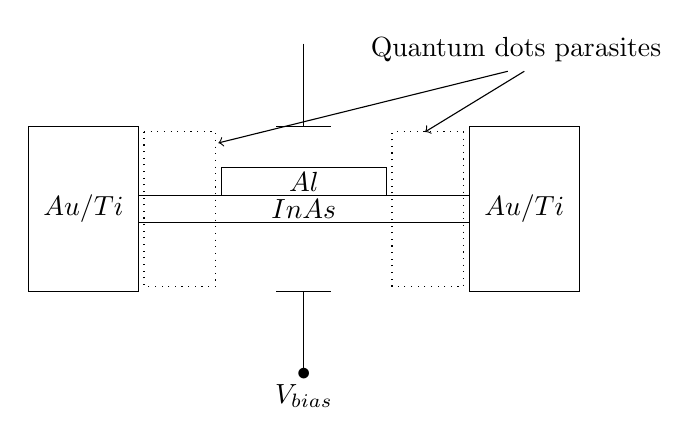
\begin{tikzpicture}[scale=0.7]
            \draw (2,0.25)--(2,-0.25)--(8,-0.25)--(8,0.25)--cycle;
            \draw (5,0)node{$InAs$};
            \draw (3.5,0.25)--(6.5,0.25)--(6.5,0.75)--(3.5,0.75)--cycle;
            \draw (5,0.5)node{$Al$};
            \draw (0,-1.5)--(0,1.5)--(2,1.5)--(2,-1.5)--cycle;
            \draw (1,0)node{$Au/Ti$};
            \draw (10,1.5)--(10,-1.5)--(8,-1.5)--(8,1.5)--cycle;
            \draw (9,0)node{$Au/Ti$};
            \draw (5,3)--(5,1.5);
            \draw (4.5,1.5)--(5.5,1.5);
            \draw (5,-3)--(5,-1.5);
            \draw (4.5,-1.5)--(5.5,-1.5);
            \draw [dotted] (2.1,1.4)--(3.4,1.4)--(3.4,-1.4)--(2.1,-1.4)--cycle;
            \draw [dotted] (7.9,1.4)--(7.9,-1.4)--(6.6,-1.4)--(6.6,1.4)--cycle;
            \draw [<-] (3.45,1.2)--(8.7,2.5);
            \draw [<-] (7.2,1.4)--(9,2.5);
            \draw (8.85,2.5)node[above]{Quantum dots parasites};
            \draw (5,-3) node{$\bullet$} node[below]{$V_{bias}$};
            \end{tikzpicture}
        \caption{Schéma en coupe représentant la structure réalisée à Copenhague}
        \label{StructureCopenhague}
        \vspace{1cm}
        \centering
           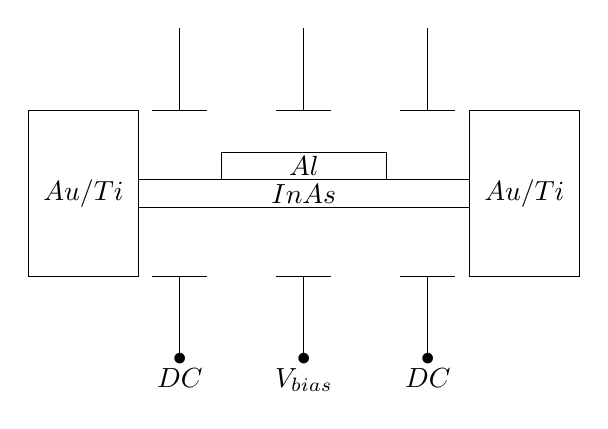
\begin{tikzpicture}[scale=0.7]
            \draw (2,0.25)--(2,-0.25)--(8,-0.25)--(8,0.25)--cycle;
            \draw (5,0)node{$InAs$};
            \draw (3.5,0.25)--(6.5,0.25)--(6.5,0.75)--(3.5,0.75)--cycle;
            \draw (5,0.5)node{$Al$};
            \draw (0,-1.5)--(0,1.5)--(2,1.5)--(2,-1.5)--cycle;
            \draw (1,0)node{$Au/Ti$};
            \draw (10,1.5)--(10,-1.5)--(8,-1.5)--(8,1.5)--cycle;
            \draw (9,0)node{$Au/Ti$};
            \draw (5,3)--(5,1.5);
            \draw (4.5,1.5)--(5.5,1.5);
            \draw (5,-3)--(5,-1.5);
            \draw (4.5,-1.5)--(5.5,-1.5);
            \draw (2.75,3)--(2.75,1.5);
            \draw (3.25,1.5)--(2.25,1.5);
            \draw (2.75,-3)--(2.75,-1.5);
            \draw (3.25,-1.5)--(2.25,-1.5);
            \draw (7.25,3)--(7.25,1.5);
            \draw (6.75,1.5)--(7.75,1.5);
            \draw (7.25,-3)--(7.25,-1.5);
            \draw (6.75,-1.5)--(7.75,-1.5);
            \draw (5,-3) node{$\bullet$} node[below]{$V_{bias}$};
            \draw (7.25,-3)node{$\bullet$} node[below]{$DC$};
            \draw (2.75,-3)node{$\bullet$} node[below] {$DC$};
            \end{tikzpicture}
        \caption{Schéma en coupe représentant la structure réalisée à Copenhague après ajout de capacités de polarisation de quantum dots}
        \label{StructureCopenhagueDéfauts}
        \end{figure}
        
\chapter{Wrong measurement method}

\section{Bad pattern}
\label{badtests}


\section{Bad way of measuring}

\label{badmeasures}

\chapter{Failed Samples}
\section{Failure due to plasma}
\label{badplasma}
The plasma sometimes had some troubles and did not work properly. In the report there were the good samples but the plasma often burned the resist so that the copper evaporation could not be done properly.

\section{Failure due to EBL}
